\chapter{Improving SAT-to-Ising}
\label{cha:QAcore}

This chapter will suggest a novel algorithm to refine the encoding and retrieve a more stable solution, starting from the weaknesses put in evidence in chapter 4. 

\section{Algorithm}

The goal of postprocessing is the re-definition of the Ising encoding, modifying offset, biases and couplings between qubits so that the longer chains are reduced in size. Since all nodes that make up the chain are linked by couplings whose value is $-1$, we will ensure to modify these weights; in addition to that, we will force these nodes in using their unused couplings when possible. \\
The only way to achieve this task not altering the original SAT formulation is to re-compute the scores of each chunk of the simplified formula, defining new OMT problems that involve the additional qubits. In more details, given two penalty functions encoded in a quantum annealer architecture linked by a chain:
\begin{figure}[t]
	\begin{center}
	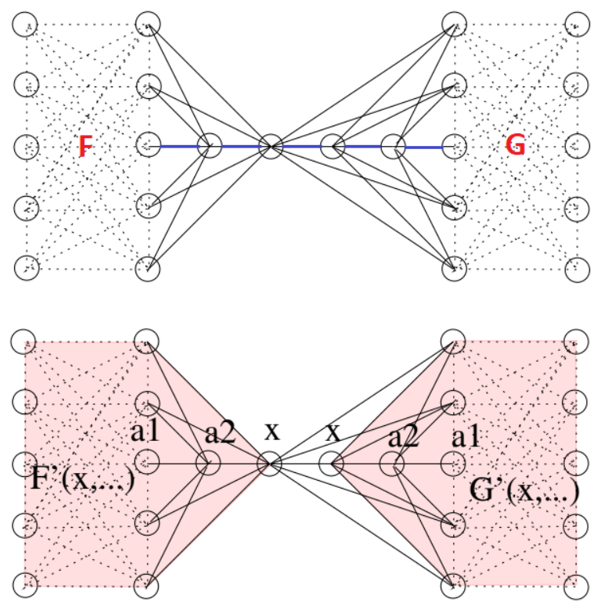
\includegraphics[]{images/Immaginetesi.png}
	\caption{A graphical representation of the postprocessing algorithm involving two general penalty functions (F and G) linked by a chain (blue edges). It is important to notice the swap of role between the original node representing the shared variable to ensure consistency of the variable's truth assignment between functions.}
	\end{center}
\end{figure}

\begin{itemize}
    \item We split the chains into two disjoint sets of nodes. The first set will be associated to the first penalty function, the second to the other.
    \item We use nodes composing the original penalty functions and the newly assigned qubits of the chain to calculate again the weights of. In particular, we use the nodes belonging to the chain as ancillas for the new function, forcing each coupling between chain nodes and penalty function qubits to be different from zero. We need also to set the most external node of the chain as the actual shared variable, so that we ensure that there is a way to link qubits representing the same Boolean variable and enforcing their equality.
    \item At this point, we have obtained a subgraph of the original architecture referring to the same. To compute new weights for, we will again rely on formula, but the presence of new ancillas will help us in reducing the number of coupling with score -1. These weights are then used to modify the Ising encoding before being passed as input to the annealer.
\end{itemize}

A graphical representation of the algorithm is shown in figure 5.1.
Post-processing cannot be applied to every quantum architecture. In order to be successful, it is necessary that qubits presents an high numbers of connections with other qubits. If this condition is not satisfied, we will not obtain great results from the re-computation of scores for penalty functions: nodes belonging to the chain will not link with external qubits and no new couplings to consider will emerge. D-Wave currently proposes two main architectures: the older one, Chimera, is clearly affected by this issue. The graph of its nodes is sparse and a qubits has at most 6 neighbour nodes, resulting in a non-valid candidate to test the novel algorithm. On the other hand the most recent architecture, Pegasus, is less sparse and it usually does not fall into the issue described above. As a consequence, from now on we will assume that the algorithm will be executed only on the Pegasus architecture.


\section{Implementation}

While the definition of the approach is linear, in practice we have to deal with numerous issues, mainly caused by computational constraints. As a consequence, the implementation relies on some heuristic that avoid apparent deadlock points during execution.
The workflow of the implementation is shown in figure 5.2.
More details on each step will be provided in the next paragraphs.

\begin{figure}[t]
	\begin{center}
	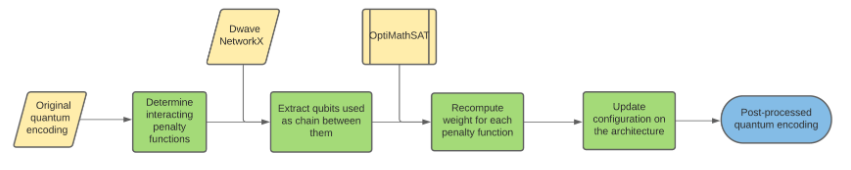
\includegraphics[width=\textwidth]{images/Workflow.png}
	\caption{A graphical representation of the workflow necessary to implement the postprocessing algorithm. Yellow nodes represent data and state-of-the-art tools; green nodes represent tasks implemented in this thesis.}
	\end{center}
\end{figure}

\subsection{Extracting encoding information}

The original version of the code returned the list of values assigned to each parameter, without any additional information about the mapping between Boolean sub-formulas and qubits. While it was not important in the precedent version, obtaining this information is now essential to determine how to rearrange qubits in new penalty functions. \\
To solve the issue, it was required to modify the \textit{place\_and\_route} library and collect data from the intermediate steps of the procedure. The routines used to determine the chosen qubits and are left unaltered; we simply added some intermediate steps which collected the missing data. In particular we first create a dictionary, called \textit{core\_penalty}, where each functions is assigned the set of qubits necessary to map it into the quantum architecture, not considering chains. We also build a second dictionary, \textit{inverted\_chains}, where the key-value items of \textit{chains} are swapped; its main role will be to quickly determine if a qubits does not represent represent a logic node and thus not considered by the procedures described in the next paragraphs.

\subsection{Re-assigning qubits}

Once the needed data are stored and available, we can start to post-process the original encoding determining what functions might be extended and what chains are involved. For each pair of penalty functions we have to determine if there is a chain connecting them which can be split in two disjoint sub-sets of qubits without altering the correctness of the encoding of the original formula. 
These operations have been implemented in the \textit{postprocessing} function. Its behaviour is explained in algorithm 1.\\
Given the set of all penalty functions, we take each possible pair and verify if there are Boolean variables shared by both of them using the field \textit{field} of the data structure \textit{penalties}. If the resulting set is empty, we can discard the couple of functions and move on the next one. In the opposite case, we call the function \textit{get\_chain} that will try to identify the chains suitable to be split. We identify the first node of the chain, represented by the qubit associated to the specified Boolean variable and contained into the \textit{core\_qubits} of the first function. From that point we recall Pegasus arcitecture from the \textbf{DwaveNetworkX} library and check if there are adjacent nodes belonging to the same chain. The new node is then added to the possible final answer and used as new middle point to search adjacent nodes, until we reach a qubits which is also part of the \textit{core\_qubits} of the second penalty function. There are some specific cases requiring exceptional handling, including:

\begin{itemize}
    \item If multiple paths arise from a single node, then we stop the search and return an empty list. The reason behind this choice is the subsequent role swap among the removed variables, which would lead to qubits on the other path to match ancillas and thus return wrong results.
    \item Similarly to the previous case, we discard also candidate chains that do not use the entire set of available qubits. In this case we know a third function shares the same variable and splitting the chain would case at least one equality with a future ancilla node. The number of times the event occurs is quite low, but it as to be taken into account to avoid unexpected behaviours.
    \item Lastly we have also to check the case in which the starting and the final node overlap. In this case we do not start the search and immediately have to return the empty list, otherwise we will reach the error case.
\end{itemize}

The backbone of \textit{get\_chain} is shown in algorithm 2. In the case a non-empty list is returned by \textit{get\_chain}, we can proceed to assign these qubits to the two penalty functions. In order to better organize the collection of the next data, a novel dictionary has been generated, called \textit{penalties\_post}. It will contain three fields for each penalty function:

\begin{itemize}
    \item \textit{nodes}, containing the list of additional qubits that we will assign to that function.
    \item \textit{edges}, containing the list of additional edges of qubits to consider in the successive steps.
    \item \textit{swap}, containing pairs of qubits whose role (ancilla/Boolean variable) need to be swapped in order to maintain the exactness of the resulting encoding, as discussed in figure 5.1.
\end{itemize}

Starting from the non-empty list of qubits, the middle point is chosen from the chain, so that two disjoint sets of nodes are generated. Qubits from the first set are progressively assigned to the first penalty function; moreover we check if there are connections among other qubits from the same penalty function not contemplated by the original problem and, when discovered, added to the \textit{edges} field. Not every node can be added: we recall from table 4.1 that at the current state we have an upper bound on the number of managed qubits to avoid deadlock points. Consequently, an additional check has been considered while scanning the list of nodes so that the upper bound is never outdated. 

\begin{algorithm}
\DontPrintSemicolon
\KwData{$penalties$ containing data about each function; \\ \qquad $chains$ containing info qubits involved in chains; \\ \qquad
$map\_arcs$ containing Pegasus graph.}
\KwResult{$p\_post$ containing data about each postprocessed function;}
\Begin{
$ub \longleftarrow 10$\;
$p\_post \longleftarrow \{\}$\;
$couples \longleftarrow \{\}$\;
\tcc{collect all possible chains between penalty functions}
\For{$f \in penalties.keys()$}{
    \For{$g \in penalties.keys()$}{
        $shared\_vars = penalties[f]["variables"] \cap penalties[g]["variables"]$\;
        \If{$shared\_vars \neq \emptyset$}{
            $couples[(f,g)] \longleftarrow shared\_vars$
        }
    }
}
\For{$c \in couples$}{
    $order\_chain = get\_chain(c, chains, penalties)$\;
    $midpoint = \left\lfloor \frac{len(order\_chain)}{2}\right\rfloor$\;
    \tcc{manipulate the first penalty function}
    \For{$i \in 1$ \KwTo $midpoint$}{
        \If{$len(penalties[c[0]]) + len(p\_post[c[0]]) > ub$}{
            \textbf{break}\;
        }
        $swap\_index \longleftarrow i$\;
        $p\_post[c[0]]["nodes"] \longleftarrow p\_post[c[0]]["nodes"] + order\_chain[i]$\;
        $adj\_nodes = map\_arcs.adjs(order\_chain[i])$\;
        \For{$qubit \in adj\_nodes$}{
            $p\_post[c[0]]["edges"] \longleftarrow p\_post[c[0]]["edges"] + (order\_chain[i], qubit)$\;
        }
    }
    $p\_post[c[0]]["swap"] \longleftarrow (order\_chain[0], order\_chain[swap\_index])$\;
    \tcc{manipulate the second penalty function}
    \For{$j \in len(order\_chain) - 2$ \KwTo $midpoint$ \KwBy $-1$}{
        \If{$len(penalties[c[1]]) + len(p\_post[c[1]]) > ub$}{
            \textbf{break}\;
        }
        $swap\_index \longleftarrow i$\;
        $p\_post[c[1]]["nodes"] \longleftarrow p\_post[c[1]]["nodes"] + order\_chain[j]$\;
        $adj\_nodes = map\_arcs.adjs(order\_chain[j])$\;
        \For{$qubit \in adj\_nodes$}{
            $p\_post[c[1]]["edges"] \longleftarrow p\_post[c[1]]["edges"] + (order\_chain[j], qubit)$\;
        }
    }
    $p\_post[c[1]]["swap"] \longleftarrow (order\_chain[len(order\_chain)-1], order\_chain[swap\_index])$\;
    }
\Return $p\_post$
}
\caption{postprocessing: qubits re-assignment}
\end{algorithm}

\begin{algorithm}
\DontPrintSemicolon
\KwData{$penalties$ containing data about each function; \\ \qquad $chains$ containing info qubits involved in chains; \\ \qquad
$map\_arcs$ containing Pegasus graph; \\ \qquad
$c$ containing the two functions involved and their shared variables}
\KwResult{$ch\_res$ containing the list of qubits for each shared variable;}
\Begin{
    $ch\_res \longleftarrow {}$ 
    \For{$var \in c$}{
        $start = chains[var] \cap penalties[c[0]]["nodes"]$\;
        $finish = chains[var] \cap penalties[c[1]]["nodes"]$\;
        \tcc{if the two functions are overimposed, we move on}
        \If{$start == finish$}{
            \Return []
        }
        $ch\_res[var] \longleftarrow start$\;
        $middle \longleftarrow map\_arcs.adjs(start) \cap chains[var]$\;
        \While{$middle$ \textbf{not in} $finish$}{
            $temp \longleftarrow map\_arcs.adjs(middle) \cap chains[var]$\;
            \tcc{if we stop prematurely or multiple paths arise, we stop}
            \If{$len(temp) \neq 1$}{
                $ch\_res[var] \longleftarrow []$\;
                \textbf{break}
            }
            $middle \longleftarrow temp$\;
            $ch\_res[var] \longleftarrow used\_nodes + middle$
        }
        \tcc{If the chain, we would case issue to the general correctness, so we skip it}
        \If{$len(ch\_res[var]) \neq len(chains[var])$}{
            $ch\_res[var] \longleftarrow []$
        }
    }
    \Return $ch\_res$
}
\caption{get\_chain}
\end{algorithm}

\subsection{Recomputing penalty functions}

In order to generate the OMT instance necessary to recompute the parameters on the enhanced penalty functions, we need to build the quadruplets of data necessary and call the \textit{searchPF} function using them as argument.\\
The easiest arguments to obtain are $n_x$ and $n_a$: the data structures $penalties$ and $penalties_post$ contain the involved nodes for each function. In details, $n_x$ can be quickly retrieved counting the number of Boolean variables from \textit{penalties}, while $n_a$ is calculated subtracting $n_x$ from the total number of qubits associated to a specific function. \\
To build the graph representing the interconnection among the nodes, we mainly rely on \textit{penalties\_post}. We instantiate a number of nodes equal to the number of needed qubits. Since the common identifiers of Pegasus nodes are not acceptable by \textbf{NetworkX} (each nome is represent by a quadruplet of integers), we converted them so that they can be mapped into integer number within the range $[0, n_a + n_x[$. This useful mapping is also stored into a dictionary, \textit{pegasus\_to\_basic}, simplifying the role swap process. Using the novel nomenclature, we define the essential edges from both \textit{penalties} and \textit{penalties\_post}. Lastly, we apply the role swap between the most external ancillas and the variable nodes, adapting \textit{pegasus\_to\_basic} so that it can reflect the update. \\
The most difficult task is the definition of the correct relation to use as reference when determining constraints on OMT decision variables. The goal is achieved thanks to the introduction of a procedure, \textit{create\_relation}. The algorithm uses the field \textit{form} coming from the genlib file as initial reference, then adapt it so that it satisfies the SMT-LIB standard and correctly refers to the right qubits. Some of the decisive operations involve:

\begin{itemize}
    \item As a preliminary step, if the genlib chosen at execution is the one accepted by Pegasus, we translate the name of the involved variables in order to use the nomenclature accepted by the Chimera genlib. This task gives us the opportunity to generalize the algorithm and not interfere with the execution of the code when Chimera is chosen as quantum architecture.
    \item Change each Boolean operator of the initial reference so that it is represented using Python symbols (for instance we rewrite each \textbf{+} into its equivalent representation \textit{or}).
    \item Combining \textit{pegasus\_to\_basic} and the field \textit{variables} of \textit{penalties}, we translate each generic variable into its equivalent node of the graph, making sure the role swap is taken into consideration.
\end{itemize}

The output of the procedure, which was a string, is lastly fed to the Python \textit{eval} function with the aim that a Boolean object is returned. \\
We also tried to enhance the actual encoding, modifying the definition of the SMT file. Two fundamental directions have been followed. First, we avoided the creation of useless decision variables, such as couplings whose value is set to zero because of architecture constraints. Instead of generating these parameters and waste resources, we extended the class of architectural constraints so that if the edges was not in the original graph, then we can immediately skip to the following one. \\
The second direction tried to exploit the formulation of a subset of decision variables defined as the weighted sum of some parameters. Instead of setting them using a combination of declaration of variable and assertion to set its value, we define each variable using \textit{let expressions}. Let expressions provide the ability to make expressions more compact by
abbreviating common sub-expressions and could impact on the time complexity, albeit slightly.

\subsection{Updating the configuration}

Once we retrieve the parameters for each recomputed penalty function, it is necessary that the quantum encoding reflects these modifies. We decided to rewrite the entire formulation of the problem from scratches, discarding the values of parameters obtained by the old version of the algorithm. Similarly to the original algorithm, we consider the updated chains setting the respective couplings as -1 and progressively increasing the offset by 1 for each edge. After this, for each function we scan the output of the OMT problem and update each parameter accordingly. The OMT solver considers the nomenclature adopted by \textbf{NetworkX}, so results are not ready to be used: the manipulation of \textit{pegasus\_to\_basic} helps us in determining what qubits are involved and what parameters need to be modified. 

\subsection{Validating the final result}

The final output provided by the quantum annealer is a dictionary containing the truth assignment for each qubit and the resulting energy as a float number. From equation 3.5 we know that if the final state reach an energy equal to zero we should obtain a satisfiable assignment; on the other hand, an energy higher than 2 indicates an unsatisfiable solution. When using the postprocessing algorithm in its early stages we could not ensure to satisfy this fundamental property; the presence of bugs could lead to the zeroing of the Hamiltonian state with a wrong assignment or the exact opposite. For this reason, additional validation has been provided thanks to the development of an algorithm which test both the old and the post-processed encoding and determining the truth value of the reported solutions. The main interest was the generation of an automatized approach, instead of manually verify the validity or \\
To accomplish this task, it was required to define a SAT problem: we decided to use OptiMathSAT as SAT solver and, consequently, we needed to write this file under the SMT-LIB standard. Each file is characterized by two main sections:

\begin{itemize}
    \item The definition of each Boolean variable and its truth value assignments.
    \item The definition of the Boolean formula we decided to test.
\end{itemize}

Regarding the first task, we simply needed to scan the returned dictionary and, for each qubits, determine if it was used as an ancilla (and thus its value was not relevant to verify the correctness) or it was yet part of the chains. In the previous steps a data structure, \textit{removed\_ancillas}, 
collects the information, so we only have to check if the qubits belong to this list. In the case of a positive outcome, we discard it and go on: on the other end we determine the physical Boolean variable associated to that node using the \textit{chains} dictionary and declare it using the structure:

\begin{equation*}
    \textbf{define-fun $<$variable name$>$ () Bool $<$true/false$>$}
\end{equation*}

Regarding the second task, we recall how \textit{penalties} collects information about each encoded penalty function, in particular storing the reference Boolean formula represented inside the field \textit{form}. We used this field as the basis for the assertions, then we adapt it replacing the general variables with the one involved in a specific function and modifying the Boolean operators so that they can match the SMT-LIB standard. \\
The two outputs have been merged into a single string variable and then fed to OptiMathSAT, which provided in response the satisfiability of the generated assignment.

\newpage

